\documentclass{standalone}
 
\usepackage{tikz}
\usetikzlibrary{automata, positioning}
\usetikzlibrary{shapes,snakes}

 \usepackage{color}
\newenvironment{gtext}{\color{gray}}{\ignorespacesafterend}
\newenvironment{btext}{\color{black}}{\ignorespacesafterend}
\definecolor{Set1_5_red}{HTML}{E41A1C}
\definecolor{Set1_5_blue}{HTML}{377EB8}
\definecolor{Set1_5_green}{HTML}{4DAF4A}

\begin{document}
    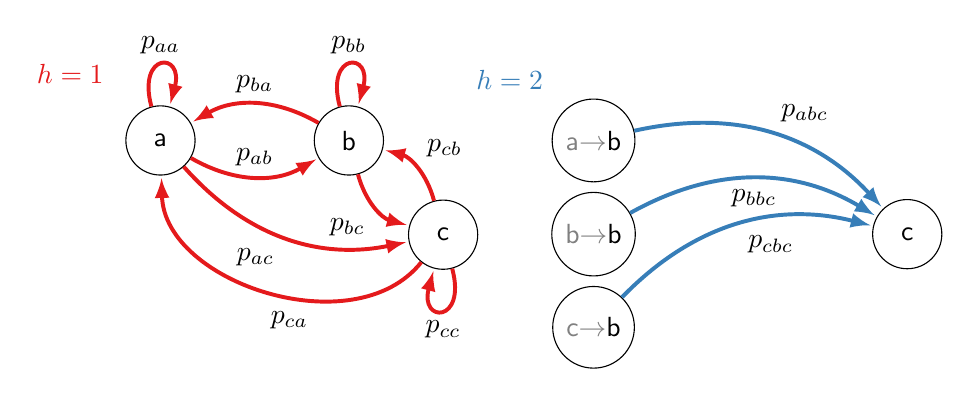
\begin{tikzpicture}[font=\sffamily]
 \begin{scope}[name=q1]
    % Add the states
    \node[state,
          text=black ] (a) {a};
    \node[state,
          right=1.5cm of a,
          text=black] (b) {b};
 \node[state,
          below right= 0.8cm of b,
          text=black] (c) {c};
  \node[above left = 0.4cm of a,color=Set1_5_red] {$h=1$};
 
    % Connect the states with arrows
    \draw[every loop,
          auto=right,
          line width=0.5mm,
          >=latex,
          draw=Set1_5_red,
          fill=Set1_5_red]
        (a) edge[bend right, auto=left]  node {$p_{ab}$} (b)
        (b) edge[bend right, auto=right] node {$p_{ba}$} (a)
         (c) edge[bend right, auto=right] node {$p_{cb}$} (b)
         (b) edge[bend right, auto=right] node {$p_{bc}$} (c)
           (c) edge[bend right = -70, auto=left,pos=0.35 ] node {$p_{ca}$} (a)
  (a) edge[bend right, auto=right] node {$p_{ac}$} (c)
        (a) edge[loop above]             node {$p_{aa}$} (a)
        (b) edge[loop above]             node {$p_{bb}$} (b)
        (c) edge[loop below]             node {$p_{cc}$} (c);
\end{scope}

\begin{scope}[xshift = 5.5cm]
    \node[state,
          text=black ] (ab) {\gtext{a$\to$}\btext{b}};
    \node[state,
          below=.12cm of ab,
          text=black] (bb) {\gtext{b$\to$}\btext{b}};
              \node[state,
          right=3cm of bb,
          text=black] (c) {c};
 \node[state,
              below=.12cm of bb,
          text=black] (cb) {\gtext{c$\to$}\btext{b}};
  \node[above left = 0.2cm of ab,color=Set1_5_blue] {$h=2$};
  
    \draw[every loop,
          auto=right,
          line width=0.5mm,
          >=latex,
          draw=Set1_5_blue,
          fill=Set1_5_blue]
        (ab) edge[bend left, auto=left]  node {$p_{abc}$} (c)
        (bb) edge[bend left, auto=right] node {$p_{bbc}$} (c)
         (cb) edge[bend left, auto=right] node {$p_{cbc}$} (c);

\end{scope}

%\begin{scope}[yshift = -4cm]
%    \node[state,
%          text=black ] (aab) {\gtext{a$\to$a$\to$}\btext{b}};
%    \node[state,
%          below=.12cm of aab,
%          text=black] (abb) {\gtext{a$\to$b$\to$}\btext{b}};
%              \node[state,
%          right=3cm of abb,
%          text=black] (ccc) {c};
% \node[state,
%              below=.12cm of abb,
%          text=black] (acb) {\gtext{a$\to$c$\to$}\btext{b}};
%
%  
%      \node[state, right=7.5cm of aab,
%          text=black ] (cab) {\gtext{c$\to$a$\to$}\btext{b}};
%    \node[state,
%          below=.12cm of cab,
%          text=black] (cbb) {\gtext{c$\to$b$\to$}\btext{b}};
%              \node[state,
%          right=3cm of abb,
%          text=black] (ccc) {c};
% \node[state,
%              below=.12cm of cbb,
%          text=black] (ccb) {\gtext{c$\to$c$\to$}\btext{b}};
%          
%%%%%%%%%%%%%%%%%%%%%%%%%%%%%%%
%     \node[state, below=2cm of ccc,
%          text=black ] (bbb) {\gtext{b$\to$b$\to$}\btext{b}};
%    \node[state,
%           left=.62cm of bbb,
%          text=black] (bab) {\gtext{b$\to$a$\to$}\btext{b}};
%  \node[state,
%             right=.62cm of bbb,
%          text=black] (bcb) {\gtext{b$\to$c$\to$}\btext{b}};          
%          
%  \node[above left = 0.15cm of aab,color=Set1_5_green] {$h=3$};
%  
%    \draw[every loop,
%          auto=right,
%          line width=0.5mm,
%          >=latex,
%          draw=Set1_5_green,
%          fill=Set1_5_green]
%        (aab) edge[bend left, auto=left]  node {$p_{aabc}$} (ccc)
%        (abb) edge[bend left, auto=right] node {$p_{abbc}$} (ccc)
%         (acb) edge[bend left, auto=right] node {$p_{acbc}$} (ccc)
%        (cab) edge[bend right, auto=right]  node {$p_{cabc}$} (ccc)
%        (cbb) edge[bend right, auto=right] node {$p_{cbbc}$} (ccc)
%         (ccb) edge[bend right, auto=right] node {$p_{ccbc}$} (ccc)
%         (bab) edge[bend left, auto=left,pos=0.2]  node {$p_{babc}$} (ccc)
%        (bbb) edge[] node {$p_{bbbc}$} (ccc)
%         (bcb) edge[bend right, auto=right] node {$p_{bcbc}$} (ccc);
%\end{scope}

   \end{tikzpicture}
\end{document}